\documentclass{article}
\usepackage{hyperref}
\usepackage{pgfplots}
\usepackage{array}
\usepackage{booktabs, caption}
\usepackage[flushleft]{threeparttable}
\usepackage{float}
\usepackage[top=2.5cm, bottom=2.5cm, left=2.5cm, right=2.5cm]{geometry}

\pgfplotsset{width=10cm}

\bibliographystyle{IEEEtran}

\title{DV2551 - 3D Programming III \\
	\large Performance Testing
	}

\author{Christoffer Bohman \\
	MScEng: Game Engineering \\
	Blekinge Institute of Technology \\
	\\
	Contact: \\
	chbh22@student.bth.se / student@skyh1gh.dev \\
	}

\date{\today}

\begin{document}

\maketitle

\newpage

\section{Introduction}

Vulkan and DirectX 12 are both newer graphics APIs that let the programmer work on a lower level than ever before. They not only allow the developers to structure their rendering
system in a variety of ways, but also enable deeper optimisations of it compared to OpenGL and previous DirectX iterations. However, as a result of this freedom, the ability
to ``shoot yourself in the foot'' also increases significantly. With this in mind, it is crucial that a wide range of tools and programs need to be accessible for the programmer
in order to maximise the potential of these graphical programming interfaces. In this report, we will be diving deeper into one such tool, namely Nvidia Nsight Graphics which 
traces and tracks the GPUs behaviour during the runtime of graphical code.

\section{Method}

\subsection{Specifications}

\begin{itemize}
	\item \textbf{Operating System} - Windows 11 (Ver 25H2, Build 10.0.26200)
	\subitem{\textbf{Version} - 25H2}
	\subitem{\textbf{Build} - 10.0.26200}

	\item \textbf{Central Processing Unit} - Intel(R) Core(TM) Ultra 9 285
	\subitem{\textbf{Cores (Performance / Efficient)}} - 24 (8 / 16)
	\subitem{\textbf{Threads}} - 24
	\subitem{\textbf{Base Clock (Performance / Efficient)}} - 1.9GHz / 2.5GHz
	\subitem{\textbf{Turbo Clock (Performance / Efficient)}} - 4.6GHz / 5.4GHz

	\item \textbf{Graphics Processing Unit} - NVIDIA GeForce RTX 5070
	\subitem{\textbf{Driver Version} - 581.95}
	\subitem{\textbf{Cores (Shader / Ray-Tracing)} - 6144 / 48}
	\subitem{\textbf{Clock Speeds (Base / Turbo)} - 2.32GHz / 2.51GHz }
	\subitem{\textbf{VRAM Capacity} - 12GB}
	\subitem{\textbf{Memory Speed} - 28 Gb / s}
	\subitem{\textbf{Bandwidth} - 672 GB / s}

\end{itemize}

\subsection{Methodology}

The testing done for this assignment was done through Nvidia Nsight Graphics on a Windows 11 machine. The specific performance testing scenario was of the DirectX 12 API along with
an instancing stress test with a range of between 1000 to 20000 instanced rotating cubes at differing resolutions. The data collection was done through the GPU-trace feature listed
on the application which hooks the GPU debugger to the instancing performance test. The dataset was systematically collected by manually capturing each configuration of resolution
and block count through the built-in block count adjustment on top of the reset functionality that recreated each block at the center, making it possible to capture a frame with
all blocks within the viewport of the camera.

The data was then analysed frame-by-frame through the GUI provided by the Nvidia Nsight Graphics program. As this is mainly a performance test and optimisation exercise, the data that
was extracted focuses on parameters that occupy a large procent of the rendering pipeline. The data was then compiled and visualised as to help with the reasoning behind optimisation
possibilities. As to make the data as applicable as possible, Vertical Sync was also forced off in order to simulate a full capacity load.

\section{Results}

\begin{center}
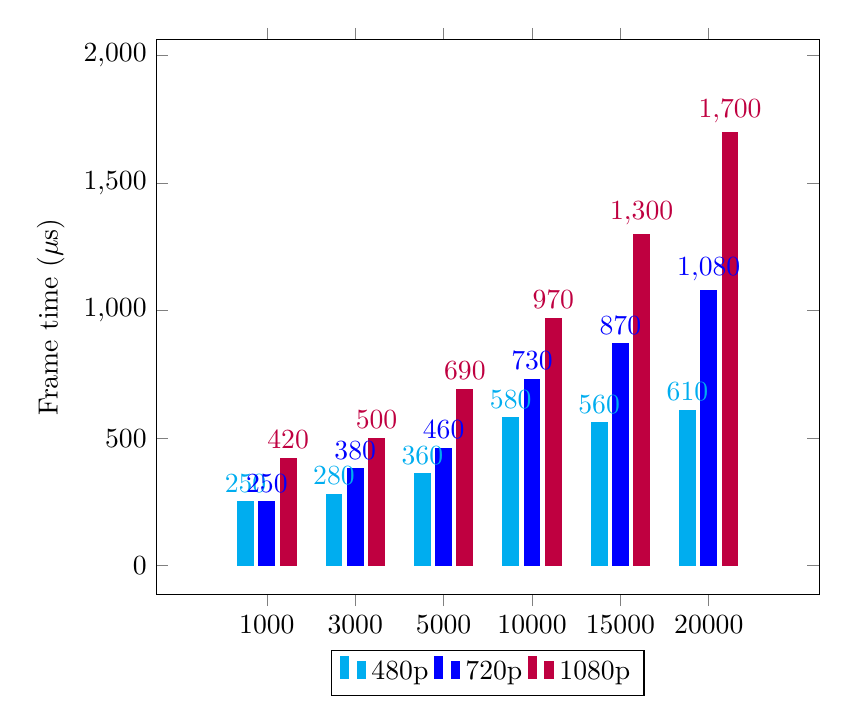
\begin{tikzpicture}
\begin{axis}[
	ybar,
	symbolic x coords={1000, 3000, 5000, 10000, 15000, 20000},
	ylabel=Frame time ($\mu$s),
	xtick=data,
	enlargelimits=0.25,
	legend style={at={(0.5,-0.1)},
	anchor=north,legend columns=-1},
	nodes near coords,
	nodes near coords align={vertical},
	bar width=0.2cm,
]
\addplot[color=cyan, fill=cyan] coordinates {(1000, 250) (3000, 280) (5000, 360) (10000, 580) (15000, 560) (20000, 610)};
\addplot[color=blue, fill=blue] coordinates {(1000, 250) (3000, 380) (5000, 460) (10000, 730) (15000, 870) (20000, 1080)};
\addplot[color=purple, fill=purple] coordinates {(1000, 420) (3000, 500) (5000, 690) (10000, 970) (15000, 1300) (20000, 1700)};


\legend{480p, 720p, 1080p}
\end{axis}
\end{tikzpicture}

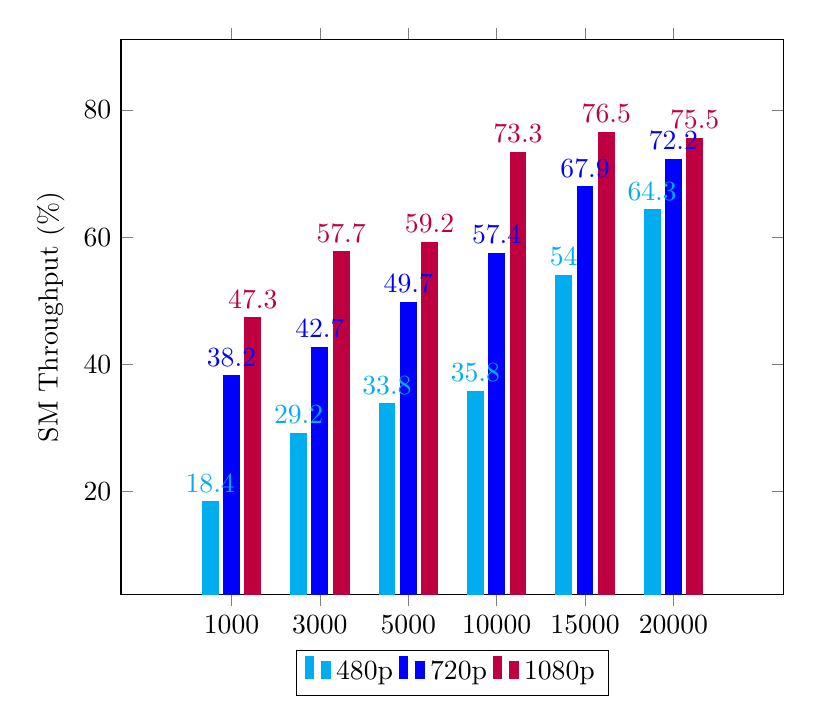
\begin{tikzpicture}
\begin{axis}[
	ybar,
	symbolic x coords={1000, 3000, 5000, 10000, 15000, 20000},
	ylabel=SM Throughput (\%),
	xtick=data,
	enlargelimits=0.25,
	legend style={at={(0.5,-0.1)},
	anchor=north,legend columns=-1},
	nodes near coords,
	nodes near coords align={vertical},
	bar width=0.2cm,
]
\addplot[color=cyan, fill=cyan] coordinates {(1000, 18.4) (3000, 29.2) (5000, 33.8) (10000, 35.8) (15000, 54.0) (20000, 64.3)};
\addplot[color=blue, fill=blue] coordinates {(1000, 38.2) (3000, 42.7) (5000, 49.7) (10000, 57.4) (15000, 67.9) (20000, 72.2)};
\addplot[color=purple, fill=purple] coordinates {(1000, 47.3) (3000, 57.7) (5000, 59.2) (10000, 73.3) (15000, 76.5) (20000, 75.5)};


\legend{480p, 720p, 1080p}
\end{axis}
\end{tikzpicture}

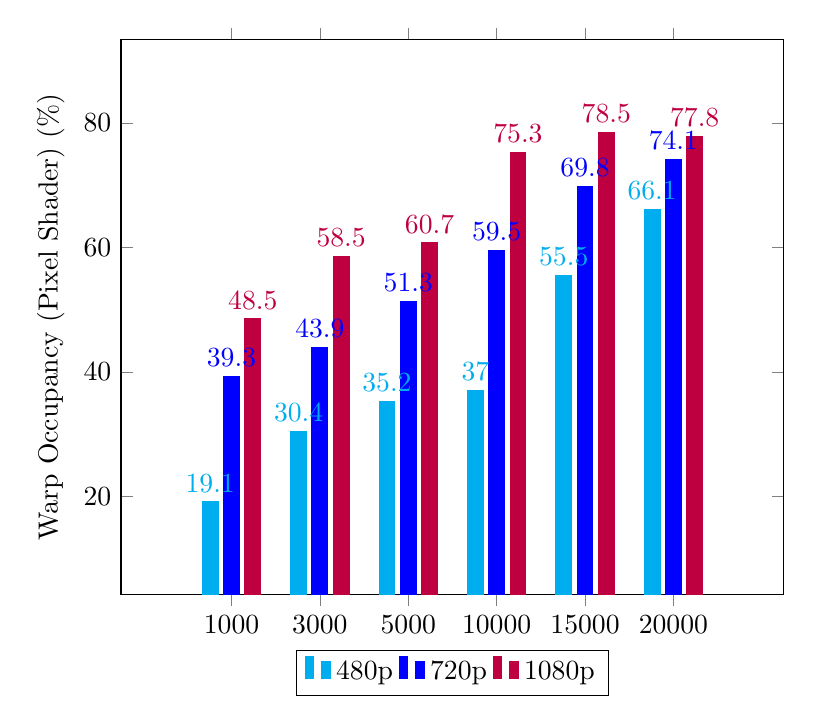
\begin{tikzpicture}
\begin{axis}[
	ybar,
	symbolic x coords={1000, 3000, 5000, 10000, 15000, 20000},
	ylabel=Warp Occupancy (Pixel Shader) (\%),
	xtick=data,
	enlargelimits=0.25,
	legend style={at={(0.5,-0.1)},
	anchor=north,legend columns=-1},
	nodes near coords,
	nodes near coords align={vertical},
	bar width=0.2cm,
]
\addplot[color=cyan, fill=cyan] coordinates {(1000, 19.1) (3000, 30.4) (5000, 35.2) (10000, 37.0) (15000, 55.5) (20000, 66.1)};
\addplot[color=blue, fill=blue] coordinates {(1000, 39.3) (3000, 43.9) (5000, 51.3) (10000, 59.5) (15000, 69.8) (20000, 74.1)};
\addplot[color=purple, fill=purple] coordinates {(1000, 48.5) (3000, 58.5) (5000, 60.7) (10000, 75.3) (15000, 78.5) (20000, 77.8)};


\legend{480p, 720p, 1080p}
\end{axis}
\end{tikzpicture}
\end{center}


\section{Discussion}

\subsection{Analysis}

I have chosen to extract the data that touches on frame times, SM throughput and the distribution of the warp occupancies. The first graph, corresponding to the frame times shows 
that the hardware used did not struggle with any of the configurations, showing results well above 60 frames per second. In most general circumstances, an optimisation would most likely
not be needed as the frame times are not of a major concern. A more in-depth optimisation would be more relevant if the application would have been unable to produce results above 60
frames per second.

The second graph shows the throughput of the streaming multiprocessors that reside on the GPU. The throughput in this case can be seen more as how big the utilisation of the GPU is 
at any point in time during rendering. The data tells us that not only does resolution change the throughput, but so does the block count. However, this does not necessarily mean that
the frame times get affected by the SM throughput, as seen especially for the 480p resolution. The third graph furthers this idea by showing that a majority of the SM occupancy is 
allocated to the pixel shader warps. As the pixel shader is per pixel, the warps required will mainly scale based on resolution.

Furthering upon the trend that the pixel shader stands for a majority of the SM usage, I delved into the pixel shader code in order to try to determine what could affect performance.
My first thought would be to try and rewrite the pipeline to be a deferred pipeline, making use of the compute shaders available to calculate all the different lighting calculations 
that occur when increasing the block count as it should lessen the load on the pixel shading step. On top of this, a good point would be to address the issues of why the SM throughput
is reaching max capacity. At a quick glance, the shader uses one float4, one float3 and two float registers, which could possibly be a contributing factor to the SM bottleneck. It could
possibly be worth to try and rewrite the code to use the caches rather than registers. There is also the possibility that this could worsen the performance as the access time of registers
is low.

\newpage

\subsection{Limitations}

Unfortunately, due to the how the machines in H470, H473 and H475 were setup, the data collection was made close to impossible as the Nvidia Nsight Graphics application requires
admin privileges for debugging which is not provided to the students. This caused me to have to move to C237 as these computers did not have these restrictions. Furthermore, I was
unable to make the shader hotspot debugging work correctly for the program, likely due to a something similar to the aforementioned problem. This also implies that my hotspot analysis
may be somewhat limited.

From a research standpoint, I would also like to point out that a more automated data collection method would prove more systematic and uniform, as the manual approach also entails
a human error factor which could affect how the rendering process looks like in for example, the pixel shader, as the cubes on screen vary based on time. An additional discussion point
could be that this simple test does not encompass any use cases where the hardware may be from an earlier generation or not as capable.

\end{document}